\documentclass[a4paper]{article}

\usepackage[intlimits]{amsmath}
\usepackage{amsthm}
\usepackage{amssymb}
\usepackage{cancel}
\usepackage{graphicx}
\usepackage{mdwlist}
\usepackage{hyperref}
\usepackage{color}
\usepackage{natbib}
\usepackage{listings}
\usepackage[nottoc,numbib]{tocbibind}

\citestyle{aa}
\bibliographystyle{apalike}

\providecommand{\e}[1]{\times10^{#1}}
\providecommand{\units}[1]{\;\mathrm{#1}}
\providecommand{\diff}[2]{\frac{\partial #1}{\partial #2}}
\providecommand{\ddiff}[2]{\frac{\partial^2 #1}{\partial #2^2}}
\providecommand{\tdiff}[2]{\frac{\mathrm{d} #1}{\mathrm{d} #2}}
\providecommand{\infint}[2]{\int\limits_{-\infty}^{\infty}{#1}\;\mathrm{d}#2}
\providecommand{\MAA}{\text{\AA}}
\providecommand{\abs}[1]{\left| #1 \right|} % for absolute value
\providecommand{\avg}[1]{\left< #1 \right>} % for average
\providecommand{\grad}[1]{\gv{\nabla} #1} % for gradient
\let\divsymb=\div
\renewcommand{\div}[1]{\gv{\nabla} \cdot #1} % for divergence
\providecommand{\curl}[1]{\gv{\nabla} \times #1} % for curl
\providecommand{\MAA}{\text{\AA}}
\providecommand{\figwidth}{.45\columnwidth}
\newcommand\numberthis{\addtocounter{equation}{1}\tag{\theequation}}
\numberwithin{equation}{section}

\providecommand{\MJ}{\ensuremath{\units{M_J}}}
\providecommand{\RJ}{\ensuremath{\units{R_J}}}
\providecommand{\MS}{\ensuremath{\units{M_\odot}}}
\providecommand{\RS}{\ensuremath{\units{R_\odot}}}

\renewcommand{\bibname}{References}

\title{Detecting Extra-Solar Planets}
\author{Tom Badran}

\date{September 2013 to May 2014}

\begin{document}

\maketitle

\tableofcontents
\listoffigures
\listoftables

\begin{abstract}
%!TEX root = project.tex
Since 1995 many extra solar planets have been discovered using the transit method. I have shown that it is possible to detect these planets using relatively low powered ground based optical telescopes (<0.5m), even under very poor seeing conditions. I also present an algorithm for analysing images and a computer program implementation of this algorithm, including an automated pipeline for processing a large sequence of images. Using this computer program, it was determined that the dwarf star, Hat P 20, has a planet of radius $(0.91\pm0.14) R_J$.

\end{abstract}

\section{Introduction}
%!TEX root = project.tex
\subsection{Motivations}

Beyond being interesting in the their own right, there are many reasons to look for, and at the properties of exoplanets. Firstly, up until the discovery of the first extra solar planetary system, PSR 1257+ 12 \citep{wolszczan1992planetary}, we were only sure of the existence of planetary bodies in our own solar system. Now we know that our system is not unusual, and it is in fact very common for stars to have many planets of their own \citep{mcarthur2004detection}, and even binary and ternary star systems to have planetary bodies \citep{marcy2002planet}.

Due to the time scales that astronomical phenomena occur on, looking at events such as star and planet formation is impossible over the lifetimes of humans, so instead we have to look at many examples of bodies at varies stages of their life cycles. By looking at planets in other solar systems we can see how they behave across different stages of their evolution, and this can be used to verify our current thinking and models for how solar systems form.

Each planet in our own system has unique and interesting properties too, so by looking elsewhere we can see how common certain characteristics are across the universe, as well as potentially discovering planets with properties completely unlike any in our own solar system.

The favourite motivator is of course the search for life beyond our own. While there is the possibility of some form of life having existed in the past on Mars \citep{mckay1996search} and the possibility of life on some of the outer moons \citep{mckay2005possibilities}, the potential of finding any kind of life, and especially multi-cellular life and even potentially intelligent life is a huge incentive. As techniques for discovering these planets have improved, there have also been observations of Earth sized planets in the so called habitable zone \citep{wordsworth2011gliese}, making the discovery of distant life a much greater possibility.

\subsection{Methods of Discovery}

\subsubsection{Transit Method}

\begin{figure}[ht]
    \centering
    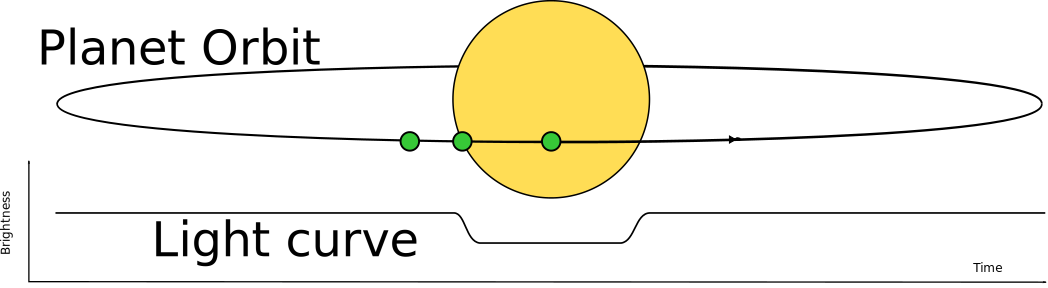
\includegraphics[width=0.8\textwidth]{images/planetary_transit.pdf}
    \caption{Example of simple model of planetary transit and the expected light curve}
    \label{fig:transit}
\end{figure}

By observing the flux from a star over period of time, any orbiting planet that passes in front of the star will cause a slight dip in the observed flux. This change in the light curve allows one to calculate the relative sizes of the planet and the star.

\paragraph{Advantages:}
\begin{itemize*}
    \item Easy to Perform
    \item Can be done at optical wavelengths
    \item Planet size can be determined
    \item Information about the planet's atmosphere can be obtained \citep{fortney2006atmosphere}
\end{itemize*}

\paragraph{Disadvantages:}
\begin{itemize*}
    \item Only works if orbital plane is in line with observer
    \item High false detection rate \citep{santerne2012sophie}
    \item Poor results for red giant stars due to their variable surface brightness
\end{itemize*}

As well as determining properties of the planet from the transit, by examining the regularity of these transits it is possible to determine information about other planets in the system. This is known as the transit timing variation method.

The period ($T$) of the planetary orbit can be figured out trivially by looking at the time between light curves. However large quantities of observations need to be taken for this.

Unfortunately the transit method only works well for large planets, as the flux dip is related to the square of the ratio of the planet to star radii. For instance observing a transit of the Earth from outside our solar system would only produce a fractional drop in flux of the order of $10^5$. A small drop like that would easily be hidden within the error, which is typically of the order of $10^3$ to $10^2$, and similar to a flux drop that would be observed simply due to a large Sunspot.

Using a simple uniform disk model (described in detail later), the planet radius can be obtained as:
\[ \frac{\Delta F}{F} = \left( \frac{R_p}{R_*} \right)^2 \]
\[ \Rightarrow R_p = R_* \sqrt{\frac{\Delta F}{F}} \]

\subsubsection{Radial Velocity}

Normally we talk about planets orbiting around a star, as this model approximates what we see very well. In actual fact however, the planet and star both orbit their common center of mass. Generally this center of mass is located very close to the center of the star so the, planet orbit model works well. However the star will move slightly, and is especially noticeable for very large planets orbiting closely, so called Hot Jupiters. As the star is moving in its own orbit, small doppler shifts can be seen in the spectrum of the star. Modern spectrometers are so accurate, that even small velocities of the order of $1\units{ms^{-1}}$ can be observed \citep{ge2002externally}. Observing using this method is often called 'Doppler Spectroscopy'.

\paragraph{Advantages:}
\begin{itemize*}
    \item Works well for low mass stars
    \item Distance independent
    \item Works for larger inclination range than transit method
    \item Gives orbital radius and planetary mass
\end{itemize*}

\paragraph{Disadvantages:}
\begin{itemize*}
    \item Depends on inclination
    \item Requires high signal to noise ratio of data
    \item Requires spectrometers rather than just CCD cameras
    \item Poor results for stars with fast rotational velocities
\end{itemize*}

The radius of orbit can be calculated as:
\[r^3 =\frac{GM_*}{4\pi^2}P_*^2 \]

Which gives the orbital velocity from Newtonian mechanics as:
\[v_p =\sqrt{\frac{GM_*}{r}} \]

The planetary mass can be calculated from the radial velocity as:
\[ m_P = \frac{M_*v_*}{v_P} \]

\subsubsection{Pulsar timing}

Pulsars rotate very rapidly, and emit radio waves as they do. The regularity of these emission is so precise that even tiny variations can be used to track the motion of the neutron star. In fact the first ever extra solar planet was confirmed using exactly this method in 1992 \citep{wolszczan1992planetary}. While this method is great for finding planets, these systems are quite rare. Also, due to the special conditions required to form planets around a white dwarf, and the intense radiation emitted, life as we know it could not evolve in these systems.

\subsubsection{Direct Observation}

\begin{figure}[ht]
    \centering
    \includegraphics[width=\figwidth]{images/direct_image.png}
    \caption{Direct image of 2MASS J01033563-5515561ABb, sourced from \cite{delorme2013direct}. The green arrow shows the position of the companion, and the blue circle shows where a background source would be expected.}
    \label{fig:direct}
\end{figure}

Under the right conditions, it can be possible to now see exoplanets directly \citep{lafreniere2010directly,kuzuhara2013direct,delorme2013direct}. Obviously stars are very bright compared to their orbiting planets making this technique a bad choice for discovering earth like planets. However large planets, many times the mass of Jupiter are observable. Using a coronagraph on the telescope limits the light from the star \citep{kuchner2002coronagraph}, and observing at infra red wavelengths can overcome the relative brightness problem \citep{delorme2013direct}.

\subsection{Selection Bias}

For all of the methods discussed, they generally favour finding large planets. This obviously leads to large selection bias in our current list of known exoplanets. While planets have proven to be commonplace in the universe, our sampling doesn't provide an overall dataset that can be used to draw conclusions about how planets are generally distributed, and if planetary systems like our own are rare or very common. This is discussed further in \citep{wright2011exoplanet}. The Kepler mission however was designed to search specifically for Earth like planets, so hopefully we will have a more comprehensive planetary database in the near future.

\section{Aims and Objectives}
\begin{itemize}
\item Create a computer software to simulate the change in observed flux from a planetary transit.
\item Observe known transits from the rooftop observatory, perform all the necessary data reduction and show that it is possible to perform useful observations even with the poor seeing in Cardiff.
\item Create a computer software that performs automated aperture photometry of stars, and use this with any observational data collected.
\item Use any observations obtained and the software pipeline constructed to infer properties of the transiting planets.
\end{itemize}


\section{Model}
%!TEX root = project.tex
Model using formulae from \cite{mandel2002analytic} and constants from \cite{mohr2012codata}


\section{Observations}
%!TEX root = project.tex

\subsection{Choosing Observing Targets}

The database at \url{http://var2.astro.cz/ETD/predictions.php} currently contains all know planetary transits, and can filter potential visible transits based on location. Using this database can quickly give us observing targets and expected transit times quickly for the few opportunities we have to observe. This data is then further filtered to find transits that fit the following criteria:
\begin{itemize}
  \item Transit occurs above thirty degrees altitude
  \item Target star has an expected magnitude less than 15 (airmass less than about 2)
  \item Magnitude change of the transit is greater than 0.01
\end{itemize}

\subsection{Observing Diary}

\subsubsection*{Tuesday, 19th November, 2013}

Due to the telescope not being correctly aligned, and having no model of the sky on which to build a model for object discovery and tracking, the first thing I had to as actually get the telescope into a usable state. After following the standard procedure for powering up the dome and telescope control systems, we performed a drift alignment on the telescope.

The telescope is an f4 20" Newtonian on a fork equatorial mount. To drift align the telescope we performed the following steps.
\begin{enumerate}
    \item Manually point to a star near the meridian
    \item Swap to the cross hair high magnification eyepiece
    \item Align the cross hair on the eye piece to the center of the star using telescope control
    \item \label{align-step}Allow telescope to track for around 5 minutes
    \item Check if star is still centered along axis
    \item If not, adjust the mount calibration control for altitude or azimuth, depending on which axis we are calibrating for, and repeat from \ref{align-step}
    \item Repeat for the other axis
\end{enumerate}

After performing the drift alignment, the weather took a turn for the worse, and so were unable to complete the rest of the modeling process.

\subsubsection*{Wednesday, 20th November, 2013}

With the telescope already drift aligned, all that needed to be done is build the software calibration model used to compensate for systematic errors in the mount alignment. To do this we use a software package called T-Point. This software builds a model of the sky based on repeated alignments onto a number of known stars. 20 stars chosen across the night sky is generally considered the minimum to produce an accurate model. After building the initial model, further systematic errors, such as changes in the optical setup, can be calibrated for by building a small t-point model using a small number (around 6 or 7) known stars.

The steps required to build the model are as follows:
\begin{enumerate}
  \item Ensure the hour angle and declination are set to 2.0 and 0 respectively in the telescope control software
  \item Flash these values to the mount firmware
  \item Ensure clock and location settings are as accurate as possible
  \item Request telescope to slew to home location
  \item \label{slew-star}Slew to the nearest easily identifiable star, ensuring the mount doesn't flip
  \item Center the star in the eyepiece, adjusting using only the telescope control joystick
  \item Save this star into the model
  \item Repeat from \ref{slew-star} for various stars across the whole sky until the model contains at least 20 stars
  \item Save the model
\end{enumerate}

After performing this calibration on 27 stars, we then tested the model by doing some visual observations of Vega, M33 and Deneb. In each case the system found the object perfectly. Unfortunately the seeing was not good enough to attempt any photometric obvservations, and the weather was getting progressively worse throughout the evening.

\subsubsection*{Thursday, 21st November, 2013}

As we weren't familiar with the t-point software we planned on using the model again tonight. We connected the Mintron camera to the telescope eyepiece adapter, and connected the video output of the camera a splitter so we had a video signal in the dome, and one in the telescope control room.

First we slewed the telescope to Vega, and it was off by a small amount, which was to be expected as this was a different observing night. However we mistakenly re-synced the mount coordinates, rather than just adding new stars to small temporary t-point model. Unfortunately this shifted our model by approximately three arc minutes. When re-syncing again it shifted the model by a further 3 arc minutes, leaving objects well beyond the field of view of the camera. There was no way to fix this we could find, and unfortunately it seems we have to disregard the model we made and create a new one.

After a few hours experimenting with trying to fix the setup, the sky became overcast and we were unable to continue.

\subsubsection{Reuse of previous observational data}

Unfortunately due to the terrible weather this winter, I have been unable to collect any data of my own. However I was able to obtain the images taken by Chris Fuller on the 23rd of March 2011 for use in his undergraduate work. Starting with these unprocessed fits, I was able to apply the pipeline I created and generate a light curve, which will be discussed later.

\section{Data processing pipeline}
%!TEX root = project.tex
\subsection{Image Correction}

\begin{figure}[ht]
    \centering
    \begin{minipage}[b]{\figwidth}
        \centering
        \includegraphics[width=\textwidth]{images/bias.png}
        \caption{Sample bias image generated with our equipment}
        \label{fig:bias_image}
    \end{minipage}\quad\quad
    \begin{minipage}[b]{\figwidth}
        \includegraphics[width=\textwidth]{images/flat.png}
        \caption{Sample flat image generated with our equipment}
        \label{fig:flat_image}
    \end{minipage}
\end{figure}

\begin{figure}[ht]
    \centering
    \begin{minipage}[b]{\figwidth}
        \centering
        \includegraphics[width=\textwidth]{images/raw_image.png}
        \caption{Uncorrected image from the CCD}
        \label{fig:raw_image}
    \end{minipage}\quad\quad
    \begin{minipage}[b]{\figwidth}
        \includegraphics[width=\textwidth]{images/corrected_image.png}
        \caption{Image after applying bias and flat correction}
        \label{fig:corected_image}
    \end{minipage}
\end{figure}

\subsubsection{Bias Image}

Firstly, systematic errors in the optical equipment need to be accounted for. Initially a correction needs to be made for the noise in the CCD electronics. To do this a set of images are taken with the shortest possible exposure time (0 seconds if possible). Then an average is built from this set of images. This data is then subtracted from any image taken using the CCD to get an image without the noise. An example bias image taken with our SBIG CCD can be seen in figure \ref{fig:bias_image}.

\subsubsection{Flat Image}

Secondly, we have to account for varying sensitivity across the CCD. Under normal circumstances, even with an even distribution of light, a CCD will not react perfectly evenly. Essentially there will be a regions of higher and lower sensitivity, and even the best CCD's will have a variation of the order of a few percent. This will have a big impact on our photometry readings as objects move within the frame, as we are looking for flux changes of only a few percent. To correct for this, we take images against a clear patch of sky that will ideally be evenly lit. These images are then averaged. Then, this final average is normalised, and then any image taken by the CCD can be divided by this flat image, after correcting for noise.

\subsubsection{Summary}

So in summary, after creating a bias and a flat image, and image taken by the CCD can be corrected by first substracting the bias image, and secondly dividing by the flat image. Bias and flat images need to be recreated throughout an observing session if possible to compensate for CCD temperature changes. A raw uncorrected image can be seen in figure \ref{fig:raw_image}, and after applying bias and flat correction can be seen again in \ref{fig:corected_image}.

\subsection{Object Detection}

\begin{figure}[ht]
    \centering
    \includegraphics[width=0.85\textwidth]{images/starfinder.png}
    \caption{Corrected image shown with the locations of stars discovered by the software. Red markers show stars found}
    \label{fig:finder_image}
\end{figure}

The first step in performing automated photometry is to actually identify. The common method to find objects in an astronomical image is to use the sextractor tool \citep{bertin1996sextractor}. However as this software is a bit of a black box, I chose to also experiment with writing my own tool to find stars. The pipeline is written to support using both the sextractor tool and my own algorithm interchangeably. Configuration information provided to the sextractor tool can be found in the appendices. An image showing the accuracy of the star finder can be seen in figure \ref{fig:finder_image}.

\subsubsection{Algorithm for star detection}

The algorithm I devised was designed to be as simple as possible, and perform quickly on a large fits images. While code for the algorithm can be found in the listing in the appendix, here is a simple description of the method:
\begin{enumerate}
    \item Estimate the background level
    \item Find local maxima above this background, with SNR above some given threshold
    \item With these maxima locations, perform a 2D gaussian fit around the region to find the center of the object
\end{enumerate}

The final gaussian fit gives both the center of the star with sub pixel accuracy, and a good estimate of the radius of the star by using the FWHM of the gaussian.

\subsection{Object Tracking}

The optical setup and mount alignment are never perfect, so stars will drift inside the field of view. As we are collecting data over a period of the order of around 4 hours for most transitions, stars may have moved by as much as a few hundred pixels between the initial and final image in the sequence.

Objects in the image don't just drift, there will also be some rotation due to imperfect mount alignment. Over the course of an observing session this may be as much as a few degrees. For stars towards the edge of the frame, this could be a large pixel distance on the image.

Luckily, both of these operations are easy to describe mathematically, and thus easy to numerically fit for. Traditionally image transformations in computers are described as a translation, rotation, and scale. In this case, we can disregard any scale change and just concentrate on the translation and rotation transformations.

Rotation is described by the matrix operation:
\[
\begin{bmatrix}
    u \\ v
\end{bmatrix}
=
\begin{bmatrix}
\cos\theta & -\sin\theta \\
\sin\theta & cos\theta
\end{bmatrix}
\begin{bmatrix}
    x \\ y
\end{bmatrix}
\]

The translations is described by:
\[
\begin{bmatrix}
    u \\ v
\end{bmatrix}
=
\begin{bmatrix}
    \Delta x \\ \Delta y
\end{bmatrix} +
\begin{bmatrix}
    x \\ y
\end{bmatrix}
\]

The total change from image to image is then described by the sum of both of these operations. A very simple tracking algorithm can then be constructed by simply using a least squares fit on the data by performing both operations, and attempting to minimise the total pixel difference when subtracting one image from the other. As stars are much brighter than the background, this function will be minimized when the stars lie on top of each other as much as possible. The changes from image to image are small enough so that it doesnt matter which order the operators are applied. For larger drifts this would not be the case as the rotation would no longer be approximately around a fixed point, and a more complex function would be required to describe the change.
\[
\begin{bmatrix}
    u \\ v
\end{bmatrix}
=
\begin{bmatrix}
\cos\theta & -\sin\theta \\
\sin\theta & cos\theta
\end{bmatrix}
\begin{bmatrix}
    x + \Delta x \\ y + \Delta y
\end{bmatrix}
\]

\subsection{Photometry}

To perform photometry, we simply want to calculate the flux of the star. With both a location and estimated radius for the star, this is trivial to obtain. The total flux is simply the sum of the flux inside an aperture with radius of the star, minus the background within the aperture.

\begin{figure}[ht]
    \centering
    \includegraphics[width=0.85\textwidth]{images/airmass.png}
    \caption{Observational parameters of the star Wasp-33}
    \label{fig:airmass}
\end{figure}

Firstly, an airmass correction can be performed. Most visible transits happen across a range of altitude, and many of the stronger ones are low in the sky. An example of a star with a transit can be seen in figure \ref{fig:airmass}. The airmass can be corrected for simply by normalising for an airmass of one at the zenith, so the airmass is given simply by $\sec \theta$, where $\theta$ is the altitude of the object.

While this gives us flux values for each star, they are not calibrated and so a further calibration step must be performed. This is done by using calibration stars in the same frame, that should be chosen not to be variable.
\[ \text{Calibrated} = \frac{\text{Measured Flux}}{\text{Calibration Star Flux}} \]

This can be performed with many calibration stars to compensate for both not always knowing if a star is a variable, and  differences in seeing across the field of view.

\bibliography{references}

\break
\appendix
\addcontentsline{toc}{section}{Appendices}

%!TEX root = project.tex

\providecommand{\pycode}[3]{
  \subsection{#1}
  \lstinputlisting[title=#3, breaklines=true, basicstyle=\scriptsize\ttfamily, numbers=left, tabsize=4,language=Python]{#2}
}

\providecommand{\configfile}[1]{
  \lstinputlisting[breaklines=true, basicstyle=\scriptsize\ttfamily, numbers=left, tabsize=4]{#1}
}
\section{Code Listings}

\pycode{Main Pipeline}{../pipeline.py}{pipeline.py}
\pycode{Uniform Disk Model}{../model/uniform_disk.py}{model/uniform\_disk.py}
\pycode{Quadratic Limb-Darkening Model}{../model/quad_limb.py}{model/quad\_limb.py}
Large portions of code in this file was sourced from \citep{mandel2002analytic}.
\pycode{File modification time dependency checking}{../common/dependency.py}{common/dependency.py}
\pycode{Fits Image Display and Data Visualisation}{../common/display.py}{common/display.py}
\pycode{Gaussian fitting routines}{../common/gaussian.py}{common/gaussian.py}

\section{SExtractor Configuration}

\configfile{../config.sex}


\end{document}
